\documentclass[10pt]{article}
\usepackage{graphicx}
\usepackage[utf8]{inputenc}
\usepackage[T1]{fontenc}
\usepackage[brazilian]{babel}
\usepackage{comment} 
\usepackage{geometry}
\geometry{
    a4paper,
    total={170mm,257mm},
    left=20mm,
    top=20mm,
 }
\setlength{\parindent}{4em}
\setlength{\parskip}{1em}
\renewcommand{\baselinestretch}{1.2}

\title{Listão P2 Redes}
\author{Guilherme Christopher Michaelsen Cardoso}

\begin{document}

\maketitle

\begin{enumerate}
    \item Conceitue a gerência de redes OSI com detalhes (mostrando desenhos)
    com os principais componentes e da arquitetura de gerência OSI). Quais
    são as principais características da gerência de redes SNMP (considere
    também os conhecimentos adquiridos na realização do segundo trabalho
    prático)? \\
    \par\textit {
        \underline{Gerência de Redes} é uma aplicação distribuída, onde 
        processos de gerência (agente-gerente) trocam informações entre si
        com o objetivo de monitorar e controlar a rede. O 
        \underline{Processo Gerente} envia solicitações ao 
        \underline{Processo Agente}, que por sua vez responde as solicitações
        e envia notificações ao processo gerente. Para responder as solicitações
        o Processo Agente consulta uma MIB, ou seja, uma Base de
        Informações Administrativas, onde ficam armazenadas as informações
        da rede que são estruturadas em forma de árvore, seguindo o 
        \underline{paradigma de orientação a objetos}, onde objetos gerenciados
        representam os recursos da rede. 
    }
    \begin{figure}[h!]
        \centering
         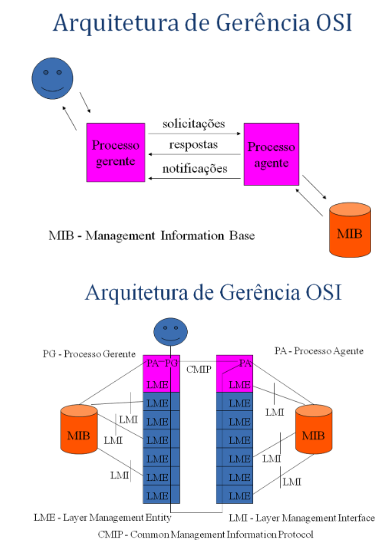
\includegraphics[width=80mm]{figura.png}
        \label{fig:figuragay}
    \end{figure}

    \item Comente sobre as cinco áreas funcionais da gerência de redes e
    serviços (Gerência de Configuração, Falhas, Desempenho, Segurança e
    Contabilidade), considerando ai mplantação e uso de uma rede de computadores
    em conformidade com o plano de negócios(atividades) da empresa(instituição).

    \item Comente sobre as sete unidades de dados do protocolo ou operações de
    gerência de redes do SNMP (Simple Network Management Protocol): GetRequest,
    SetRequest, GetNextRequest, GetBulkRequest, Response, Trap e InformRequest

    \item Comente sobre os primeiros RFCs (Request for Comments) para o SNMP, 
    também conhecido como SNMPv1, que apareceram em 1988: (RFC 1065- Structure
    and identification of management information for TCP/IP-based internets;
    RFC 1066 - Managemetn information base for network management of TCP/IP
    based internets; RFC 1067 - A simple network management protocol)

    \item Apresente os elementos de serviços da camada de aplicação OSI envolvidos 
    com as operações de gerência de redes e as respectivas primitivas relacionadas
    com a operação de gerência GET

    \item Comente sobre os três principais modelos de serviços e os quatro modelos
    de implantação relacionados com computação em nuvem (cloud computing).

    \item Comente sobre as funções das três principais camadas (view, integration
    and infrastructure layers) da arquitetura PCMONS (Private Cloud Monitoring
    System).

    \item Descreva sucintamente as atividades relacionadas ao projeto e desenvolvimento
    de protocolos (especificação informal, especificação formal, validação, 
    verificação, implementação e teeste) descrevendo as relações existentes entre estas
    atividades. Para explicitar melhor, apresente também um desenho destas atividades e
    relações \textbf{(não, não apresento, vsf)}.

    \item Observe a especificação através de modelos de transição [MEF (Maquina 
    de Estados Finitos)] realizada abaixo para o protocolo de enlace de dados entre
    as duas interfaces de uma rede local, onde o controle de fluxo empregado é do tipo
    envia-espera e após enviar um quadro de dados a emissora aguarda a chegada do seu
    reconhecimetno.
    \begin{enumerate}
        \item Considerando a transmissão de um QU (Quadro de Usuário) da máquina 1 
        para máquina 2 descreva o que acontece em cada transição realizada pelas MEF,
        citando os elementos dos conjuntos de entrada e saída envolvidos, desde
        o recebimento de QU no BE1 da máquina 1 até o recebimento do ACKIN no BE2 da
        máquina 1.
        \item Considerando a chegada de DADOIN na máquina 2, mostre como é acionada
        a "temporização" na máquina 1 e reenviado o DADOOUT, apresentando as transições
        com seus respectivos elementos dos conjuntos de entrada e saída da MEF 
        envolvidos; também explique sobre o que acontece na ocorrência de cada 
        transição. 
        \item Comente sobre alguns problemas que podem ocorrer devido a simplicidade 
        deste protocolo (MEF), mostrando as transições com seus respecitvos elementos
        dos conjuntos de entrada e saída da MEF envolvidos para o exemplo de duplicação
        de dados recebidos.
        \begin{figure}[h!]
            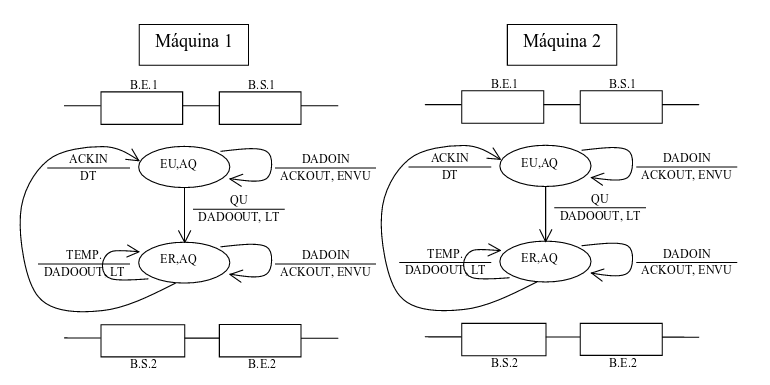
\includegraphics[width=\linewidth]{mef.png}
            \label{fig:mef1}
        \end{figure}
    \end{enumerate}
    \item O emprego de Modelos de Transição como técnica de especificação formal de
    protocolas apresenta alguns problemas. Para auxiliar nesta situação são utilizados
    também Linguagens de Programação e Modelos Mistos. Cite alguns problemas, 
    descrevendo em que sentidos as Linguagens de Programação e os Modelos Mistos podem
    auxiliar. Como as ferramentas de especificação formal, Lotos, Estelle, Z..., podem
    auxiliar para resolver os problemas os problemas mencionados acima?

    \item Concluída a verificação de especificação de um protocolo, chega o momento
    de implementá-lo nos vários sistemas da rede que irão utilizá-lo em suas 
    comunicações. A decisão de como integrar a implementação de um protocolo no 
    sistema local se assenta nos seguintes objetivos, relativos ao nível de desempenho
    desejado: minimizar custo do serviço de comunicação; maximizar vazão nas conexões
    utilizadas; minimizar a utilização dos recursos do sistema dedicados à comunicação.
    Tendo em vista esses objetivos, a implementação pode ser integrada de três 
    maneiras. Quais são estas maneiras? Comente um pouco sobre cada uma destas
    maneiras.

    \item Quais são as principais topologias de redes locais existentes? Apresente
    desenhos e comentários sobre as topologias relacionadas aos padrões IEEE 802.3,
    802.4 e 802.5.

    \item Comente sobre os protocolos IEEE 802.3 - CSMA/CD (Carrier Sense Multiple
    Access with Collision Detection) para barramento (apresente um fluxograma),
    IEEE 802.4 - "token bus" e IEEE 802.5 - "token ring".

    \item O que é chaveamento de pacotes e de circuitos? Comente sobre as vantagens
    de cada tipo de chaveamento.

    \item Ainda em relação a camada de rede comente sobre: roteamento, controle de 
    congestionamento, serviço não orientado e orientado a conexões. 

    \item Quantas redes estão disponíveis e quantos computadores podemos interconectar
    em cada classe de endereço (IPv4) da Internet?
\end{enumerate}
\end{document}
